\section{Durchführung}
\label{sec:Durchführung}

\subsection{Vorbereitungen vor der Messung}
\label{ssec:durch1}

Bevor der eigentliche Versuch beginnt muss die Hysteresemessung für den Elektromagneten durchgeführt werden.
Dafür wird ein Feldstrom angelegt.
Zwischen die Polschuhe des Magneten wird eine Hall-Sonde gefahren, um die Magnetfeldstärke $B$ zu bestimmen.
Nun wird der Strom $I$ erhöht und in regelmäßigen Schritten wird $B$ in Abhängigkeit von $I$ notiert. 
Anschließend wird vom Maximum aus, hier sind das $\SI{5}{\ampere}$, wieder auf $\SI{0}{\ampere}$ heruntergeregelt.

In diesem Versuch wird der Zeeman-Effekt anhand einer Cd-Lampe demonstriert.
Genauer gesagt, wird für den normalen Zeeman-Effekt die rote Linie von Cd genutzt und für den anomalen die blaue Linie.
Für beide Teile des Experiments wird der Aufbau aus \autoref{fig:aufbau} genutzt. 
\begin{figure}
    \centering
    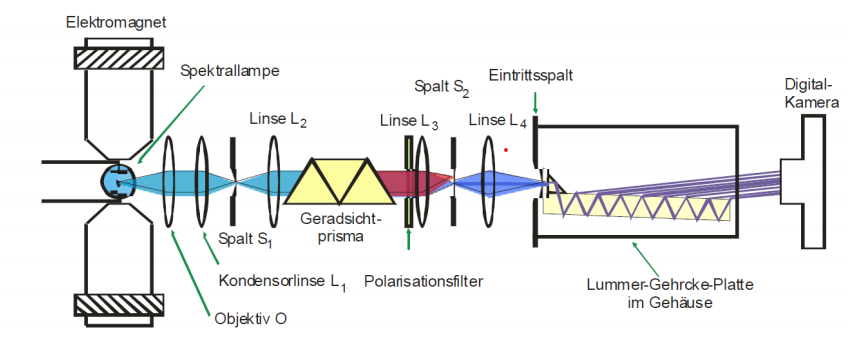
\includegraphics[width=\textwidth]{images/aufbau1.png}
    \caption{Grobe Skizze der Messapperatur. \cite{V27}}
    \label{fig:aufbau}
\end{figure}
Der Polarisationsfilter wird je nach Messung aus dem Aufbau entfernt oder umgestellt.

\subsection{Messung der roten Linie}
\label{ssec:durch2}

Die Cd-Lampe wird nun angeschaltet.
Das Licht der Lampe muss fokussiert auf den ersten Spalt treffen. 
Die Linsen und Entfernungen müssen dem entsprechend angepasst werden.
Im Gradsichtprisma wird das emittierte Licht nun in seine verschiedenen Wellenlängen aufgeteilt.
Da in dieser Messung nur die rote Linie von Interesse ist, wird der zweite Spalt so verschoben, dass nur dieser Anteil passieren kann. 
Auch hier muss darauf geachtet werden, dass das eintreffende Bild scharf abgebildet wird. 
Nach einer erneuten Fokussierung trifft das rote Licht auf die Lummer-Gehrcke-Platte und erzeugt das Interferenzbild.
Hinter der Platte steht eine Kamera mit der das Bild fotografiert werden soll, hierbei ist ein Bild zu wählen, bei dem die Abstände zwischen den Maxima gut zu sehen sind.
Im zweiten Schritt wird nun das Magnetfeld eingeschaltet. 
Die benötigte Magnetfeldstärke wird vorher über die Formel \autoref{eq:bfeld} bestimmt, alle nötigen Größen sind bekannt. 
Das Interferenzbild spaltet sich nun auf, ohne den Polarisationsfilter sollten aus einer Linie drei geworden sein.
Dieses Bild wird ebenfalls für die spätere Auswertung gespeichert.
Ein Beispiel für solche Aufnahmen ist in \autoref{fig:bild} dargestellt.
\begin{figure}
    \centering
    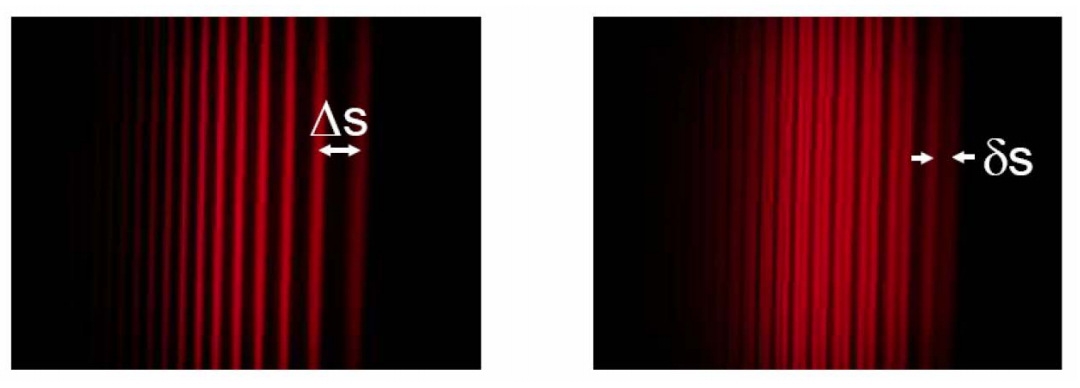
\includegraphics[width=\textwidth]{images/bild.png}
    \caption{Beispiel für ein Interferenzbild mit und ohne Magnetfeld \cite{V27}}
    \label{fig:bild}
\end{figure}

\subsection{Messung der blauen Linie}
\label{ssec:durch3}

Die grundlegende Messung lauft äquivalent zur vorherigen Messung, allerdings wird der zweite Spalt hier so eingestellt, dass nur das blaue Licht passieren kann.
In diesem Messchritt muss der Polarisationsfilter in den Aufbau integriert werden. 
Je nach Einstellung wird im Interferenzbild die $\pi$- oder die $\sigma$-Spektrallinie abgebildet. 
Eigentlich gibt es vier $\sigma$-Linien, sie liegen aber nahe beieinander und werden deshalb nur als eine dargestellt. 
Wie vorher, werden von den Interferenzbildern Fotos mit der Kamera gemacht.
Für beide Fälle wird jeweils ein Magnetfeld eingestellt, das sich wieder über \autoref{eq:bfeld} ergibt.
Auch hier werden Bilder gemacht.
